

\begin{center}
\LARGE
Delprøve med hjælpemidler 
\end{center}
\stepcounter{section}
%%%%%%%%%%%%%%%%%%%%%%%%%%%%%%%%%%%%%%%%%%%%%%%%%%%%%%%%%%%%%%%%%%%%%%%
%							Ny Opgave!!!!!							%
%%%%%%%%%%%%%%%%%%%%%%%%%%%%%%%%%%%%%%%%%%%%%%%%%%%%%%%%%%%%%%%%%%%%%%%
\begin{opgavetekst}{Opgave 1}
	En funktion $f$ er givet ved forskriften
	\begin{align*}
		f(x) = 7x-15.
	\end{align*}
\end{opgavetekst}
\begin{delopgave}{}{1}
	Bestem $f(-5)$.
\end{delopgave}
\begin{delopgave}{}{2}
	Bestem skæringenspunktet mellem grafen for $f$ og $x$-aksen. 
\end{delopgave}
%%%%%%%%%%%%%%%%%%%%%%%%%%%%%%%%%%%%%%%%%%%%%%%%%%%%%%%%%%%%%%%%%%%%%%%
%							Ny Opgave!!!!!							%
%%%%%%%%%%%%%%%%%%%%%%%%%%%%%%%%%%%%%%%%%%%%%%%%%%%%%%%%%%%%%%%%%%%%%%%
\begin{opgavetekst}{Opgave 2}
	To punkter $P$ og $Q$ er givet ved
	\begin{align*}
		&P(2,5), &&Q(6,-11).
	\end{align*}
\end{opgavetekst}
\begin{delopgave}{}{1}
	Bestem en forskrift for den lineære funktion $g$, hvis graf skærer gennem $P$ og $Q$. 
\end{delopgave}
\begin{delopgave}{}{2}
	Løs ligningen $g(x) = 10$
\end{delopgave}
\begin{meretekst}
	En anden lineær funktion $h$ er givet ved
	\begin{align*}
		g(x) = 2x+3
	\end{align*}
\end{meretekst}
\begin{delopgave}{}{3}
	Bestem koordinaterne for skæringspunktet mellem graferne for $g$ og $h$. 
\end{delopgave}
%%%%%%%%%%%%%%%%%%%%%%%%%%%%%%%%%%%%%%%%%%%%%%%%%%%%%%%%%%%%%%%%%%%%%%%
%							Ny Opgave!!!!!							%
%%%%%%%%%%%%%%%%%%%%%%%%%%%%%%%%%%%%%%%%%%%%%%%%%%%%%%%%%%%%%%%%%%%%%%%
\begin{opgavetekst}{Opgave 3}
	Jette-Bettina kører med taxafirmaet TaxA og hun vil gerne kende deres priser,  men de oplyser ikke deres priser. Hun kører derfor forskellige afstande med TaxA og nedskriver distancen hun har kørt 		samt prisen for turen. Jette-Bettina har et alkoholproblem, så hun får ikke altid noteret prisen og distancen helt korrekt, og hun antager derfor, at hun må bruge en del målinger før hun har et 		    godt datagrundlag. Hun antager desuden, at prisen $p(x)$ for at køre $x$ kilometer med taxa er givet ved en sammenhæng af typen
	\begin{align*}
		p(x) = ax+b.
	\end{align*}
	Hendes data kan ses på Tabel. \ref{tab:taxa}.
	\begin{table}[H]
		\centering
		\begin{tabular}{c|c|c|c|c|c}
			$x$ (distance i km) & 2 & 5 & 7 & 8 & 11 \\
			\hline
			$p$ (pris i kr) & 102 & 160 & 203 & 231 & 277
		\end{tabular}
		\caption{Sammenhæng mellem afstand og pris.}
		\label{tab:taxa}
	\end{table}
	\phantom{h}
\end{opgavetekst}
\begin{delopgave}{}{1}
	Brug Tabel \ref{tab:taxa} til at bestemme $a$ og $b$.
\end{delopgave}
\begin{delopgave}{}{2}
	Brug modellen til at afgøre, hvor langt Jette-Bettina kan komme for 400 kr.
\end{delopgave}
\begin{meretekst}
	Et konkurrende taxafirma TaxB har følgende model, der beskriver deres prissætning.
	\begin{align*}
		q(x) = 10x + 400,
	\end{align*}
	hvor $x$ er afstanden kørt i km og $q$ er prisen i kr. 
\end{meretekst}
\begin{delopgave}{}{3}
	Afgør, hvor langt man skal køre før at TaxA er billigst at køre med.
\end{delopgave}
%%%%%%%%%%%%%%%%%%%%%%%%%%%%%%%%%%%%%%%%%%%%%%%%%%%%%%%%%%%%%%%%%%%%%%%
%							Ny Opgave!!!!!							%
%%%%%%%%%%%%%%%%%%%%%%%%%%%%%%%%%%%%%%%%%%%%%%%%%%%%%%%%%%%%%%%%%%%%%%%
\begin{opgavetekst}{Opgave 4}
	\begin{center}
		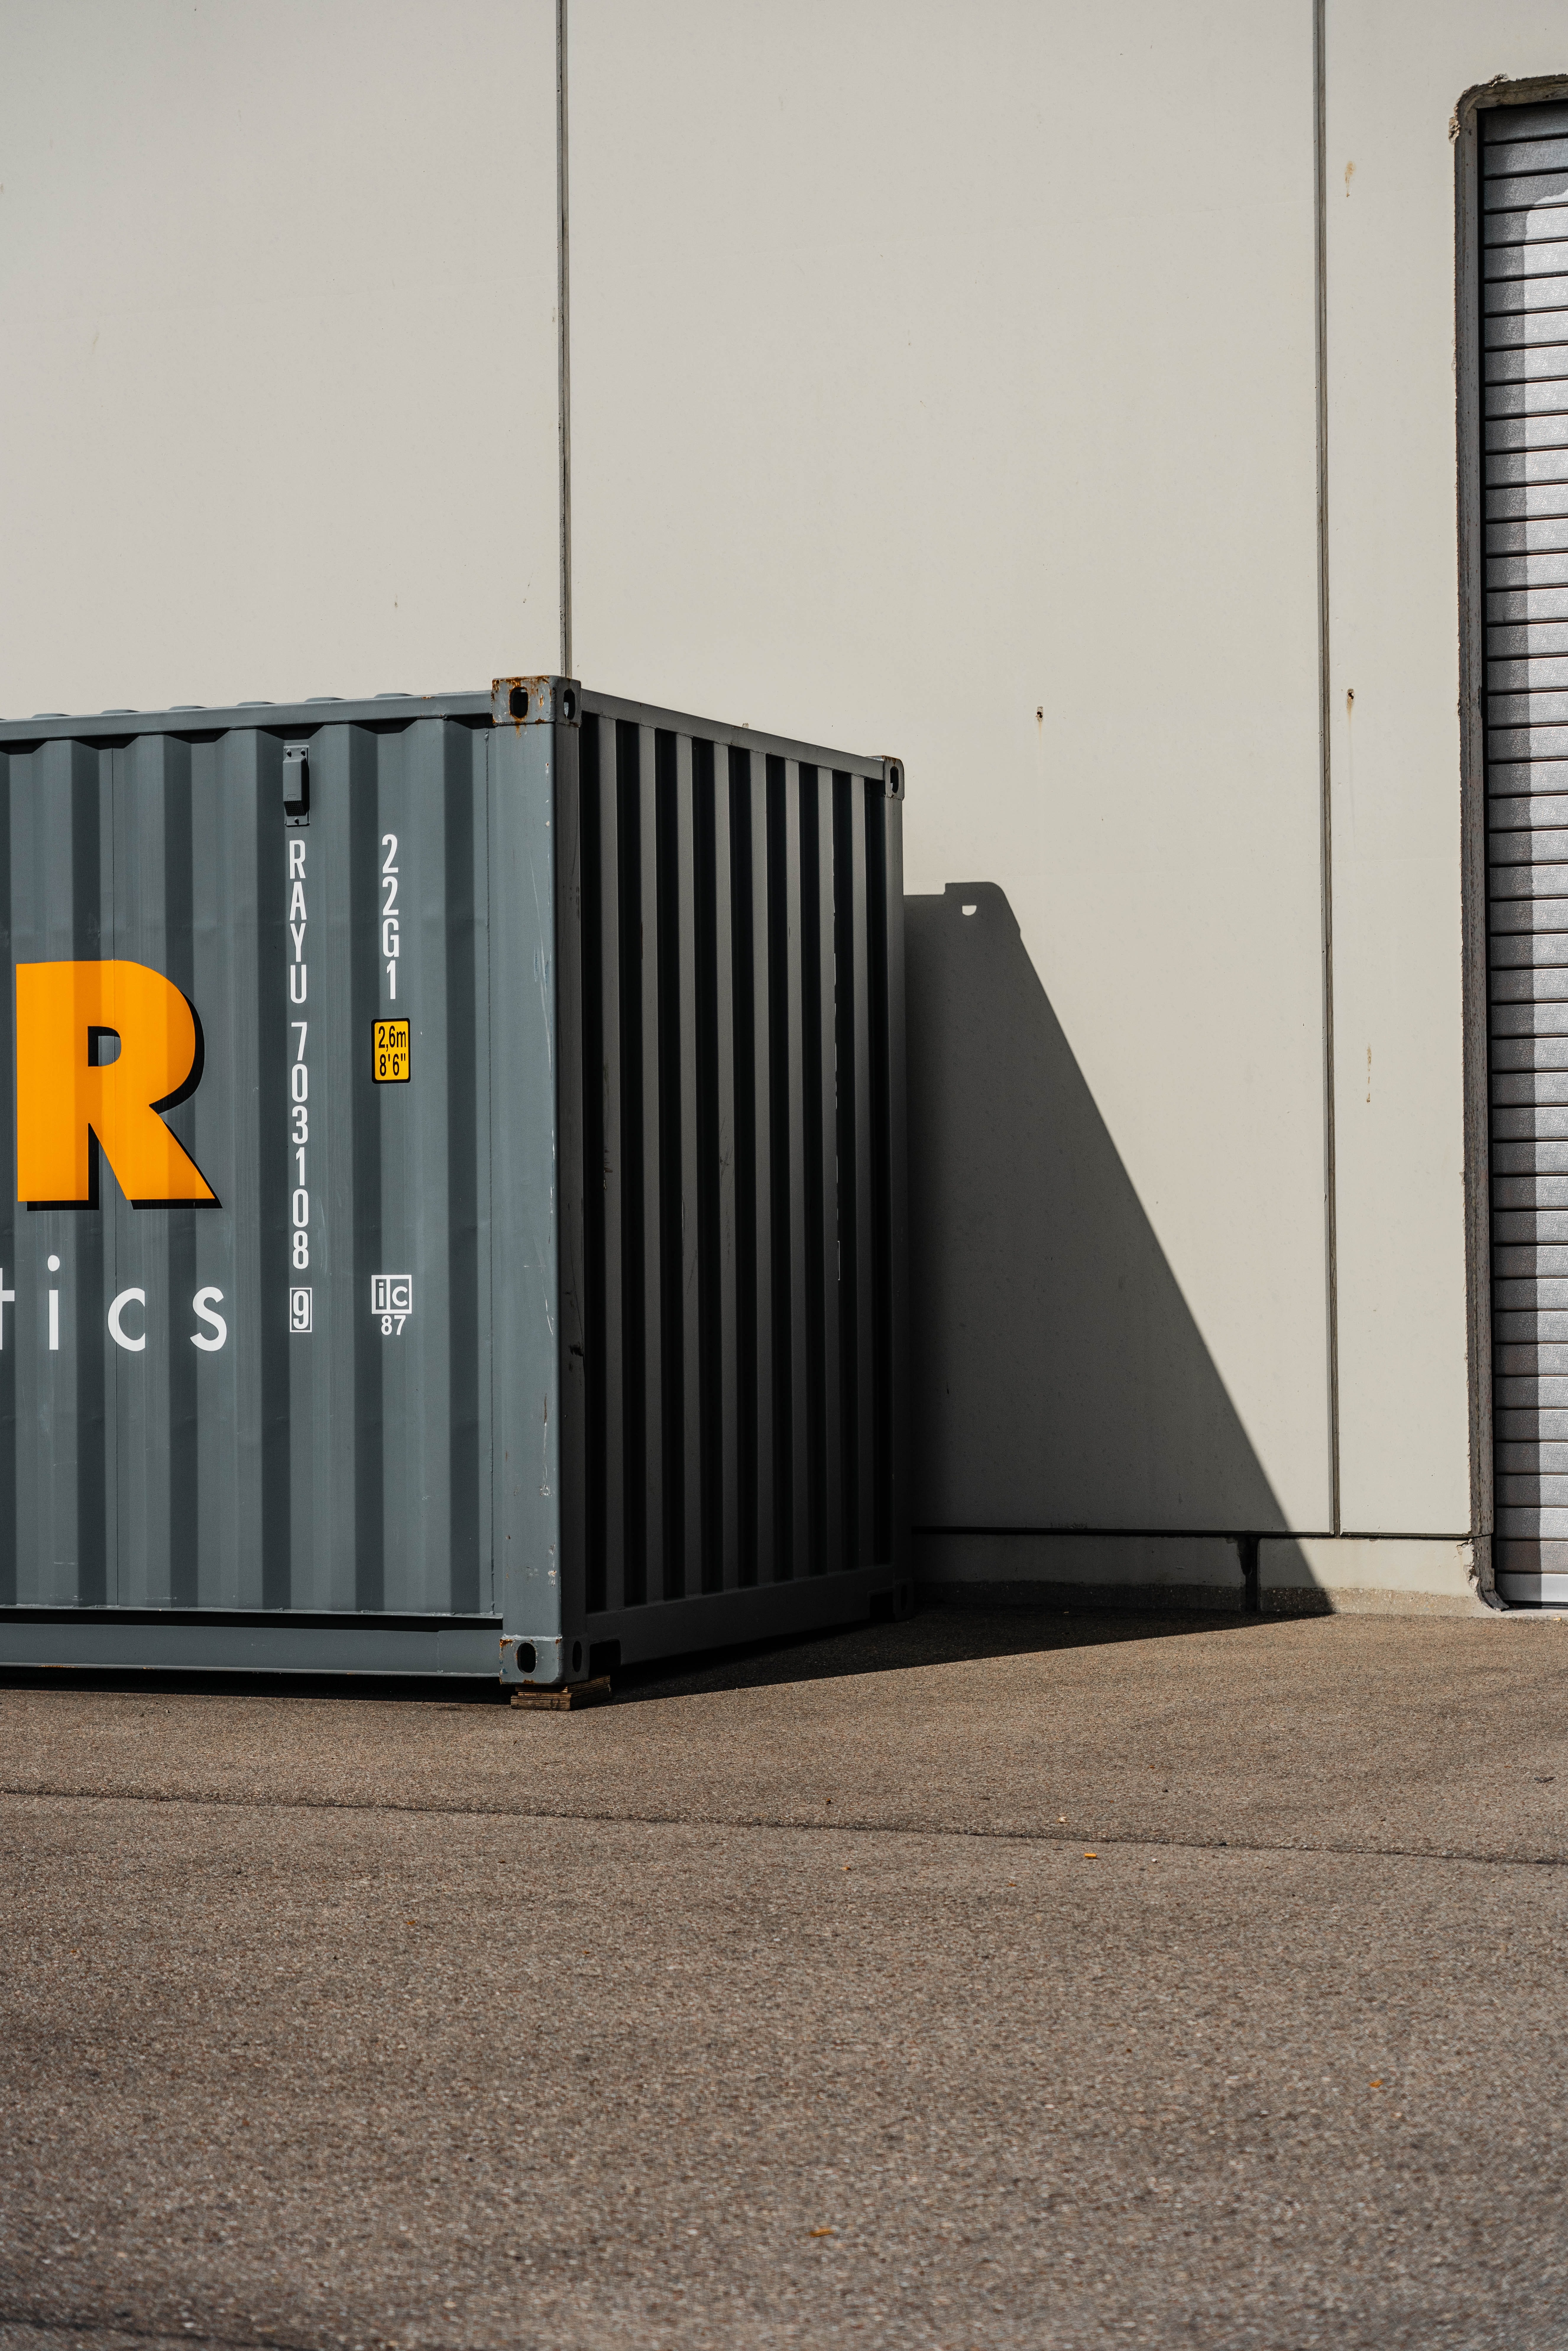
\includegraphics[width=0.4\textwidth]{Billeder/container.jpg}
	\end{center}
	En gruppe venner skal fylde sand i en container. Containeren vejer 715 kg, og de fylder 2300 kg sand i containeren i timen. 
\end{opgavetekst}
\begin{delopgave}{}{1}
	Indfør passende variable og opstil en model, der beskriver sammenhængen mellem vægten af containeren og tiden, vennegruppen har brugt på at fylde sand i containeren. 
\end{delopgave}
\begin{delopgave}{}{2}
	Bestem vægten af containeren efter tre timer. 
\end{delopgave}
\begin{meretekst}
	Én af vennerne gør de andre opmærksomme på, at den maksimale totalvægt på containeren er 10.000kg.
\end{meretekst}
\begin{delopgave}{}{3}
	Hvor længe kan de fylde sand på containeren før den overstiger maksimalvægten?
\end{delopgave}
%%%%%%%%%%%%%%%%%%%%%%%%%%%%%%%%%%%%%%%%%%%%%%%%%%%%%%%%%%%%%%%%%%%%%%%
%							Ny Opgave!!!!!							%
%%%%%%%%%%%%%%%%%%%%%%%%%%%%%%%%%%%%%%%%%%%%%%%%%%%%%%%%%%%%%%%%%%%%%%%
\begin{opgavetekst}{Opgave 5}
	Af Tabel \ref{tab:labour} kan aldersfordeling for fødende kvinder i Danmark ses.
	\begin{table}[H]
	\centering	
	\begin{tabular}{c|c|c|c|c|c|c}
		Alder (År) & 15-20 & 20-25 & 25-30 & 30-35 & 35-40 & 40-45\\
		\hline
		Frekvens & 1.9 & 16.2 & 37.7 & 32.2 & 10.5 & 1.5
	\end{tabular}
	\caption{Alder for fødende kvinder i Danmark.}
	\label{tab:labour}
	\end{table}
	\phantom{h}
\end{opgavetekst}
\begin{delopgave}{}{1}
	Tegn en sumkurve for fordelingen fra Tabel \ref{tab:labour}.
\end{delopgave}
\begin{delopgave}{}{2}
	Afgør, hvor stor en procentdel af fødende kvinder, der er under 30 år.
\end{delopgave}

\begin{opgavetekst}{Opgave 6}
	En gruppe på 15 personer har i løbet af en uge nedskrevet deres totale antal toiletbesøg. Resultatet er 
	\begin{align*}
		35,35,37,42,43,43,43,45,45,46,49,50,50,51,53,60.
	\end{align*}
\end{opgavetekst}
\begin{delopgave}{}{1}
	Bestem det gennemsnitlige antal toiletbesøg.
\end{delopgave}
\begin{delopgave}{}{2}
	Tegn et boksplot, der viser fordelingen af antallet af toiletbesøg. 
\end{delopgave}


